\definecolor{poscolor4}{HTML}{38ada9}
\definecolor{poscolor5}{HTML}{78e08f}
\definecolor{poscolor6}{HTML}{b8e994}
\definecolor{poscolor7}{HTML}{008BCC}
\definecolor{poscolor8}{HTML}{00AC53}
\definecolor{poscolor9}{HTML}{3E4372}
\begin{figure}[t]
\centering
\pgfplotsset{
    width=8cm,height=5.5cm,
    every axis y label/.append style={at={(-0.1,0.5)}},
    every axis/.append style={line width=0.6pt},
}

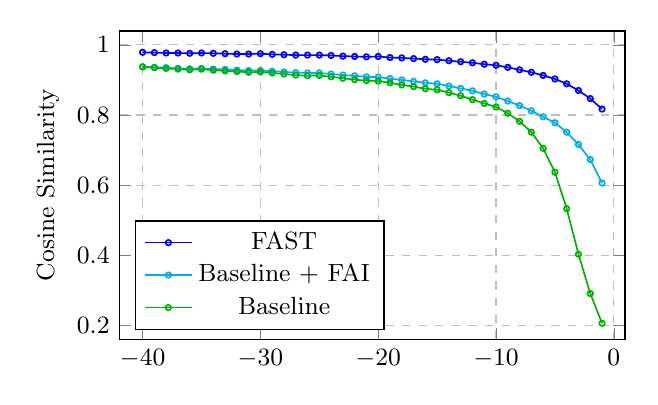
\begin{tikzpicture}[baseline]
\begin{axis}[
    ylabel=Cosine Similarity,
    enlargelimits=0.05,
    font=\small,
    legend pos=south west,
    legend style={font=\small},
    ymajorgrids=true,
    xmajorgrids=true,
    grid style=dashed,
    ymin=0.2, ymax = 1.0,
    ytick={0.2,0.4,0.6,0.8,1.0},
]
\addplot[color=blue,mark=o, mark size=1pt] coordinates{(-40,0.979)(-39,0.978)(-38,0.977)(-37,0.977)(-36,0.976)(-35,0.977)(-34,0.976)(-33,0.975)(-32,0.974)(-31,0.974)(-30,0.975)(-29,0.973)(-28,0.972)(-27,0.971)(-26,0.971)(-25,0.971)(-24,0.97)(-23,0.968)(-22,0.967)(-21,0.966)(-20,0.967)(-19,0.964)(-18,0.963)(-17,0.961)(-16,0.959)(-15,0.958)(-14,0.955)(-13,0.952)(-12,0.949)(-11,0.945)(-10,0.942)(-9,0.936)(-8,0.929)(-7,0.922)(-6,0.913)(-5,0.903)(-4,0.889)(-3,0.87)(-2,0.847)(-1,0.817)};
\addplot[color=cyan,mark=o, mark size=1pt] coordinates{(-40,0.938)(-39,0.936)(-38,0.935)(-37,0.933)(-36,0.932)(-35,0.933)(-34,0.931)(-33,0.930)(-32,0.928)(-31,0.927)(-30,0.927)(-29,0.925)(-28,0.923)(-27,0.921)(-26,0.920)(-25,0.920)(-24,0.917)(-23,0.914)(-22,0.912)(-21,0.909)(-20,0.908)(-19,0.904)(-18,0.900)(-17,0.896)(-16,0.892)(-15,0.889)(-14,0.883)(-13,0.876)(-12,0.869)(-11,0.860)(-10,0.852)(-9,0.840)(-8,0.827)(-7,0.812)(-6,0.795)(-5,0.778)(-4,0.751)(-3,0.716)(-2,0.673)(-1,0.606)};
\addplot[color=green!70!black,mark=o, mark size=1pt] coordinates{(-40,0.937)(-39,0.935)(-38,0.933)(-37,0.931)(-36,0.929)(-35,0.931)(-34,0.928)(-33,0.926)(-32,0.924)(-31,0.922)(-30,0.923)(-29,0.920)(-28,0.917)(-27,0.914)(-26,0.912)(-25,0.913)(-24,0.909)(-23,0.905)(-22,0.901)(-21,0.898)(-20,0.897)(-19,0.892)(-18,0.886)(-17,0.881)(-16,0.875)(-15,0.872)(-14,0.864)(-13,0.855)(-12,0.844)(-11,0.833)(-10,0.823)(-9,0.805)(-8,0.782)(-7,0.751)(-6,0.705)(-5,0.637)(-4,0.533)(-3,0.403)(-2,0.291)(-1,0.206)};
\legend{FAST,Baseline + FAI,Baseline,}
\end{axis}
\end{tikzpicture}
\caption{Effect on the average cosine similarity $\Bar{s}_{-t^{\prime}}$ of the streaming speech representations at the end positions (before mask tokens). After applying FAI and FAST, the representations of the end positions are improved.}
\label{fig:whywork}
\end{figure}









